%%%%%%%%%%%%%%%%%%%%%%%%%%%%%%%%%%%%%%%%%%%%%%%%%%%%%%%%%%%%%%%%%%%%%%
%
%         Copyright (c) 2023, gitlabci_gallery / latex
%         All rights reserved.
%
%%%%%%%%%%%%%%%%%%%%%%%%%%%%%%%%%%%%%%%%%%%%%%%%%%%%%%%%%%%%%%%%%%%%%%

\documentclass[A4,svgnames,9pt,aspectratio=169]{beamer}
%% document options:
%% - aspectratio = { 43, 169, 1610 }
%% - utf8
%%


\setlength{\footskip}{300pt}
\usepackage[french]{babel}

\hypersetup{
   allcolors   = rouge_inria,
   pdfauthor   = {Duzés Florian},
   pdftitle    = {\@title},
   pdfsubject  = {Point hebdomadaire, bi-mensuel du stage},
   pdfkeywords = {entretien, observation du travail}
}

%%%%%%%%%%%%%%%%%%%%%%%%%%%%%%%%%%%%%%%%%%%%%%%%%%%%%%%
%%
%%%%%%%%%%%%%%%%%%%%%%%%%%%%%%%%%%%%%%%%%%%%%%%%%%%%%%%

\title[titrecourt]{Réunion flash}
\subtitle{Point hebdomadaire}
\date[30/07/2025]{date long}
\author[Duzes Florian]{Duzés Florian}

\usetheme{inria}


\begin{document}

%%%%%%%%%%%%%%%%%%%%%%%%%%%%%%%%%%%%%%%%%%%%%%%%%%%%%%%
%%
%%%%%%%%%%%%%%%%%%%%%%%%%%%%%%%%%%%%%%%%%%%%%%%%%%%%%%%

\frame{\titlepage}

%%%%%%%%%%%%%%%%%%%%%%%%%%%%%%%%%%%%%%%%%%%%%%%%%%%%%%%

% Le titre des planches de sommaire est \contentsname, sa valeur
% est fixée ici à "Sommaire" par défaut.
\renewcommand{\contentsname}{Sommaire}

\frame{\tocpage}


%%--%%--%%--%%--%%--%%--%%--%%--%%--%%--%%--%%--%%--%%--%%
 
\section{État des lieux}
\frame{\sectionpage}

\begin{frame}{Point actuel}
  \begin{tikzpicture}[
    node distance=2cm,
    box/.style={rectangle, draw=black, thick, minimum width=3cm, minimum height=1cm, text centered, rounded corners, font=\bfseries},
    arrow/.style={->, >=Stealth, thick, draw=arrowColor},
    contentBoxDone/.style={rectangle, draw=black, thick, fill=board_lightGray!40, rounded corners, minimum width=3cm, minimum height=2cm, text width=3cm, align=center},
    contentBox/.style={rectangle, draw=black, thick, rounded corners, minimum width=3cm, minimum height=2cm, text width=3cm, align=center}
]

    % DESSINS
    \node[box, fill=faitColor] (fait) {Fait};
    \node[box, fill=enCoursColor, right=of fait] (en_cours) {En cours};
    \node[box, fill=aFaireColor, right=of en_cours] (a_faire) {Prévus};
    \draw[arrow] (fait) -- (en_cours);
    \draw[arrow] (en_cours) -- (a_faire);

    % Choses réalisées
    \node[contentBoxDone, below=0.5cm of fait] {
      \begin{itemize}
        \item Remplir les config
        \item Appel des fonctions voisines
        \item Affiner la génération des tests pour \textit{Krmllib.h} et \textit{Hacl\_Hash\_Blake2b.h}
        \item Chaîne de bout en bout x86\_64 
      \end{itemize}
      };
      
      % En cours
      \node[contentBox, below=0.5cm of en_cours, fill=enCoursColor!15] {
        \begin{itemize}
          \item étude de résultat  
          \item Couverture des architectures différentes
          \item Couverture des compilateurs
        \end{itemize}
    };

    % Point fixer
    \node[contentBox, below=0.5cm of a_faire, fill=aFaireColor!15] {
        \begin{itemize}
          \item Mémoire de stage
        \end{itemize}
    };
      \end{tikzpicture}


\end{frame}

%  .  .  .  .  .  .  .  .  .  .  .  .  .  .  .  .  .  .  %

\begin{frame}{Réalisation}
  \begin{tikzpicture}[
    node distance=2cm,
    box/.style={rectangle, draw=black, thick, minimum width=3cm, minimum height=1cm, text centered, rounded corners, font=\bfseries},
    arrow/.style={->, >=Stealth, thick, draw=arrowColor},
    contentBoxDone/.style={rectangle, draw=black, thick, fill=board_lightGray!40, rounded corners, minimum width=3cm, minimum height=2cm, text width=3cm, align=center},
    contentBox/.style={rectangle, draw=black, thick, rounded corners, minimum width=3cm, minimum height=2cm, text width=3cm, align=center}
]

    % DESSINS
    \node[box, fill=faitColor] (fait) {Fait};
    \node[box, fill=enCoursColor, right=of fait] (en_cours) {En cours};
    \node[box, fill=aFaireColor, right=of en_cours] (a_faire) {Prévus};
    \draw[arrow] (fait) -- (en_cours);
    \draw[arrow] (en_cours) -- (a_faire);

    % Choses réalisées
    \node[contentBoxDone, below=0.5cm of fait] {
      \begin{itemize}
        \item Scripts de lancement
        \item Nouvel ordinateur
        \item Sauvegarde de résultats
        \item Couverture architectures
        \item Couverture 
      \end{itemize}
      };
      
      % En cours
      \node[contentBox, below=0.5cm of en_cours, fill=enCoursColor!15] {
        \begin{itemize}
          \item Affinage de l'utilisation Binsec 
          \item Correctifs de Binsec
          \item Analyse des résultats
        \end{itemize}
    };

    % Point fixer
    \node[contentBox, below=0.5cm of a_faire, fill=aFaireColor!15] {
        \begin{itemize}
          \item Mémoire de stage
        \end{itemize}
    };
      \end{tikzpicture}

\end{frame}

%%--%%--%%--%%--%%--%%--%%--%%--%%--%%--%%--%%--%%--%%--%%

\section{Érysichthon, travaille !}
\frame{\sectionpage}

\begin{frame}{Connexion des pièces détachés}
  \centering
  \begin{tikzpicture}[auto]

    % Styles
    \tikzstyle{startstop} = [rectangle, rounded corners, minimum width=2cm, minimum height=1cm, text centered, draw=black, fill=green!30]
    \tikzstyle{process} = [rectangle, minimum width=2cm, minimum height=1cm, text centered, draw=black, fill=orange!30]
    \tikzstyle{arrow} = [thick,->,>=stealth]
    \tikzstyle{arrowred} = [thick,->,>=stealth, draw=red]
    \tikzset{zone1/.style={rectangle, rounded corners, draw=red, dashed, fill=red!10, inner sep=0.3cm}}
    \tikzset{zone2/.style={rectangle, rounded corners, draw=blue, dashed, fill=blue!10, inner sep=0.5cm, text width=3cm}}
    \tikzset{zone3/.style={rectangle, rounded corners, draw=green, dashed, fill=green!10, inner sep=0.3cm}}
    \tikzset{zone4/.style={rectangle, rounded corners, draw=green, dashed, fill=green!30!blue!5, inner sep=0.3cm}}
    
    % Noeuds
    \node (make_test) [startstop] {ANDHRÍMNIR};
    \node (test) [below of = make_test] {make\_tests};
    \node (test1) [below of=test, xshift=0.5cm, yshift=0.6cm] {\small{test1}};
    \node (test2) [below of=test1, yshift=0.6cm] {\small{test2}};
    \node (test3) [below of=test2, yshift=0.6cm] {\small{test3}};
    \node (test4) [below of=test3, yshift=0.6cm] {\small{test4}};
    \node (dots) [below of=test4, yshift=0.6cm] {\small{$\dots$}};
    
    \foreach \node in {test1, test2, test3, test4, dots} {
      \draw (test.south) |- (\node.west);
      }
      
    \node (start) [startstop, right of=make_test, yshift=2cm, xshift = 4cm] {Érysichthon};
    \node (blanc) [right of=make_test,yshift=-1cm, xshift = 2cm] {};
    \node (compilateur) [below of = start] {Compilateur};
    \node (hacl) [below of = compilateur, xshift=1cm] {\textit{\$}Hacl*};
    \node (tests) [below of = hacl, yshift = 0.3cm] {\textit{\$}tests};
    \node (binsec) [below of = tests, xshift=1cm] {\textit{\$}Binsec};
    \node (analyse) [below of = binsec, yshift = 0.3cm] {Analyse};
    % Flèches
    \draw [arrow] (compilateur.south) |- (hacl.west);
    \draw [arrow] (compilateur.south) |- (tests.west);
    \draw [arrow] (tests.south) |- (binsec.west);
    \draw [arrow] (tests.south) |- (analyse.west);

    % Zones
    \begin{scope}[on background layer]
        \node (zone2node) [zone2, fit=(start) (compilateur) (hacl) (tests) (binsec) (analyse) (make_test) (test) (test1) (test2) (test3) (test4) (dots)] {};
        \node (title) [anchor=north west] at (zone2node.north west) {\parbox{3.5cm}{\centering \Huge{\textbf{Érysichthon}}\\\scriptsize{\textit{control panel}}}};
        \node (zone_tests) [zone1, fit=(make_test) (test) (test1) (test2) (test3) (test4) (dots)] {};
        \node (zone_compilation) [zone3, fit=(start) (compilateur) (hacl) (tests) (binsec) (analyse)] {};
        \node (zone_binsec) [zone4, fit=(binsec) (analyse)] {};
    \end{scope}

    % Flèches 2
    \onslide<1>{
    \draw [arrow, dashed, opacity=0.5] (title) -- (zone_tests);
    \draw [arrow, dashed, opacity=0.5] (title) -- (zone_compilation.west);
    \draw [thick,>=stealth, dashed, opacity=0.4] (title) -- (blanc.north);
    \draw [arrow, dashed, opacity=0.5] (blanc.north) -- (zone_binsec);
    \draw [arrow, dashed, opacity=0.2] (zone_tests.north) -- (zone_compilation.west);
    }
    \onslide<2>{
    \draw [arrowred] (title.east) -- (start.west);
    \draw [arrowred, opacity=0.5] (start.south) -- (hacl);
    \draw [arrowred] (hacl.west) -- (make_test.east);
    \draw [arrowred] (make_test.east) -- (tests);
    \draw [arrowred] (tests) -- (binsec);
    }
    \end{tikzpicture}
\end{frame}
%  .  .  .  .  .  .  .  .  .  .  .  .  .  .  .  .  .  .  %

\begin{frame}[fragile]{Script de travail}
  \begin{lstlisting}[style=INIStyle, caption={./erysichthon}, gobble=4]
    $ ./erysichthon 
    Usage: ./eryshicthon ARCHI PATH_Hacl [FORCE] [PATH_Compiler]
    - FORCE - default : Os
    - PATH_Compiler - default : gcc
  \end{lstlisting}
  
\end{frame}

%  .  .  .  .  .  .  .  .  .  .  .  .  .  .  .  .  .  .  %

\begin{frame}[fragile]{Lancement de l'analyse}
  \begin{lstlisting}[style=INIStyle, caption={./test.sh}, gobble=4]
    for force in O1 O2 O3 Os Oz
    do
      ./erysichthon x86_64 $HACL $force
    done
  \end{lstlisting}
  
\end{frame}

% %%--%%--%%--%%--%%--%%--%%--%%--%%--%%--%%--%%--%%--%%--%%


\section{x86\_64, ARM, RiscV}
\frame{\sectionpage}

\begin{frame}{Le trio de tête}
  \begin{columns}
    \begin{column}{0.5\textwidth}
      \begin{center}
        \begin{block}{Module x86\_64}
          \begin{itemize}
            \item Compiler Hacl*
            \item Compilation des tests
            \item Script Binsec
          \end{itemize}
        \end{block}
      \end{center}
    \end{column}
    \pause
    \begin{column}{0.5\textwidth}
      \only<2>{
        \begin{block}{Module ARM}
          \begin{enumerate}
            \item Compiler Hacl*
            \item Compilation des tests
            \item Script Binsec
          \end{enumerate}
        \end{block}

        \begin{block}{Module RiscV}
          \begin{enumerate}
            \item Compiler Hacl*
            \item Compilation des tests
            \item Script Binsec
          \end{enumerate}
        \end{block}
      }
      \only<3>{
        \begin{block}{Module ARM}
          \begin{enumerate}
            \item Compiler Hacl*
            \item[\checkmark] Compilation des tests
            \item[\checkmark] Script Binsec
          \end{enumerate}
        \end{block}

        \begin{block}{Module RiscV}
          \begin{enumerate}
            \item Compiler Hacl*
            \item[\checkmark] Compilation des tests
            \item[\checkmark] Script Binsec
          \end{enumerate}
        \end{block}
      }
    \end{column}
  \end{columns}
\end{frame}


%  .  .  .  .  .  .  .  .  .  .  .  .  .  .  .  .  .  .  %

\begin{frame}[fragile]{Compilation de Hacl*}

  \begin{lstlisting}[style=global2, caption={./configure}, gobble=4]
    Usage: configure -target <triple>

    This script configures HACL/Evercrypt. You can specify the following options:

        -target         Specify the target triple for the build. This follows the
                        Clang target triple convention.
                        Details: https://clang.llvm.org/docs/CrossCompilation.html
                        Currently supported triples are:
                        * aarch64-none-linux-android
                        * aarch64-none-linux-gnu
                        * aarch64-apple-darwin
                        * aarch64-apple-ios
                        * x86_64-apple-ios-simulator
        --disable-bzero Do not use explicit_bzero (binary will work with an old GL-
        IBC)
        --enable-power9 Enable Power ISA v3.0 instruction set for PowerPC architec-
        ture
  \end{lstlisting}
\end{frame}

%  .  .  .  .  .  .  .  .  .  .  .  .  .  .  .  .  .  .  %

\begin{frame}[fragile]{Modification de Hacl*}

  \begin{lstlisting}[style=global2, caption={./configure}, gobble=4]
    Usage: configure -target <triple>

    This script configures HACL/Evercrypt. You can specify the following options:

        -target         Specify the target triple for the build. This follows the
                        Clang target triple convention.
                        Details: https://clang.llvm.org/docs/CrossCompilation.html
                        Currently supported triples are:
                        * aarch64-none-linux-android
                        * aarch64-none-linux-gnu
                        * aarch32-none-linux-gnu
                        * aarch64-apple-darwin
                        * aarch64-apple-ios
                        * x86_64-apple-ios-simulator
                        * x86_64-none-linux-gnu
                        * riscv64-unknown-linux-gnu
                        * riscv32-unknown-linux-gnu
        --disable-bzero Do not use explicit_bzero (binary will work with an old GL-
        IBC)
  \end{lstlisting}
\end{frame}


%%%%%%%%%%%%%%%%%%%%%%%%%%%%%%%%%%%%%%%%%%%%%%%%%%%%%%%

\section{Résultats - mémorisation et analyse}
\frame{\sectionpage}

\begin{frame}[fragile]{Des logs ...}

  \begin{block}{Conservations de traces}
    \begin{itemize}
      \item \textit{\$arch.log}
    \end{itemize}
  \end{block}
  
  \begin{lstlisting}[style=global2, caption={x86\_64.log}, gobble=4]
    Binsec ··· Hacl_Hash_SHA3_Simd256_shake128
    [checkct:result] Program status is : secure (0.652)
    Binsec ··· Hacl_Hash_SHA3_Simd256_shake128_squeeze_nblocks
    [sse:warning] Symbol state comes from the file /home/fduzes/projet_inria/erysichthon/x86_64/builds/Hacl_Hash_SHA3_Simd256_shake128_squeeze_nblocks.exe and shadows other definitions
                  Use "import <state> from FILE" to disambiguate
    [sse:warning] Symbol state comes from the file /home/fduzes/projet_inria/erysichthon/x86_64/builds/Hacl_Hash_SHA3_Simd256_shake128_squeeze_nblocks.exe and shadows other definitions
                  Use "import <state> from FILE" to disambiguate
    [checkct:result] Program status is : secure (0.263)
    Binsec ··· Hacl_Hash_SHA3_Simd256_shake256
    [checkct:result] Program status is : secure (0.623)
    Binsec ··· Hacl_Hash_SHA3_Simd256_state_free
    [sse:error] Cut path 1 (uninterpreted "Invalid replacement fallthrough") @ 0x00415970 (<free>)
    [checkct:warning] Exploration is incomplete:
    [sse:result] Value 0x64656262757473 : 0x64656262757473
    [checkct:result] Program status is : unknown (0.075)
  \end{lstlisting}

\end{frame}

%  .  .  .  .  .  .  .  .  .  .  .  .  .  .  .  .  .  .  %

\begin{frame}[fragile]{... \textit{et} des dictionnaires}
  
  \begin{block}{Mise en mémoire}
    \begin{itemize}
      \item \textit{results.json}
      \item \textit{global\_results.json}
    \end{itemize}
  \end{block}

  \begin{lstlisting}[style=global2, caption={global\_results.json}, gobble=4]
    { "$archi":
              {"$option":
                  "fun": "secure|unknown|insecure"
                  ...
                  "date" : "mm_dd_yyyy_HH_MM"
              }
    }
  \end{lstlisting}

\end{frame}



%%%%%%%%%%%%%%%%%%%%%%%%%%%%%%%%%%%%%%%%%%%%%%%%%%%%%%%

\section{Mise en pratique}
\frame{\sectionpage}

\begin{frame}{Matériel de calcul}

  \begin{columns}
    \begin{column}{0.5\textwidth}
      \begin{block}{Ordinateur personnel}
        \begin{itemize}
          \item Vivobook
          \item AMD Ryzen™ 5 3500U with Radeon™ Vega Mobile Gfx x 8
          \item Debian 12
        \end{itemize}
        \textit{Récupéré auprès de proche au début du stage.}
      \end{block}
    \end{column}
    \pause
    \begin{column}{0.5\textwidth}
      \begin{block}{Colonne INRIA}
        \begin{itemize}
          \item Dell Inc. Precision Tower 7910
          \item Intel® Xeon® E5-2620 v4 × 32
          \item Ubuntu 24.04.2 LTS
        \end{itemize}
        \textit{Récupéré après le départ d'un thésard, ça traîné au bureau.}
      \end{block}
    \end{column}
  \end{columns}
\end{frame}

%  .  .  .  .  .  .  .  .  .  .  .  .  .  .  .  .  .  .  %

\begin{frame}[fragile]{Premier lancement}
  \begin{lstlisting}[style=MakefileStyle, caption={x86\_64/Makefile}, gobble=4]
    binsec: analyse
      @binsec -sse -sse-depth 1000000 -sse-timeout 20 -sse-script $(BINSEC_SCRIPT) -checkct $(DUMP)
  \end{lstlisting}

  \pause
  L'écran se gèle. \\
  Perte de contrôle...
\end{frame}

%  .  .  .  .  .  .  .  .  .  .  .  .  .  .  .  .  .  .  %

\begin{frame}{Lancement malins}
  \begin{center}
    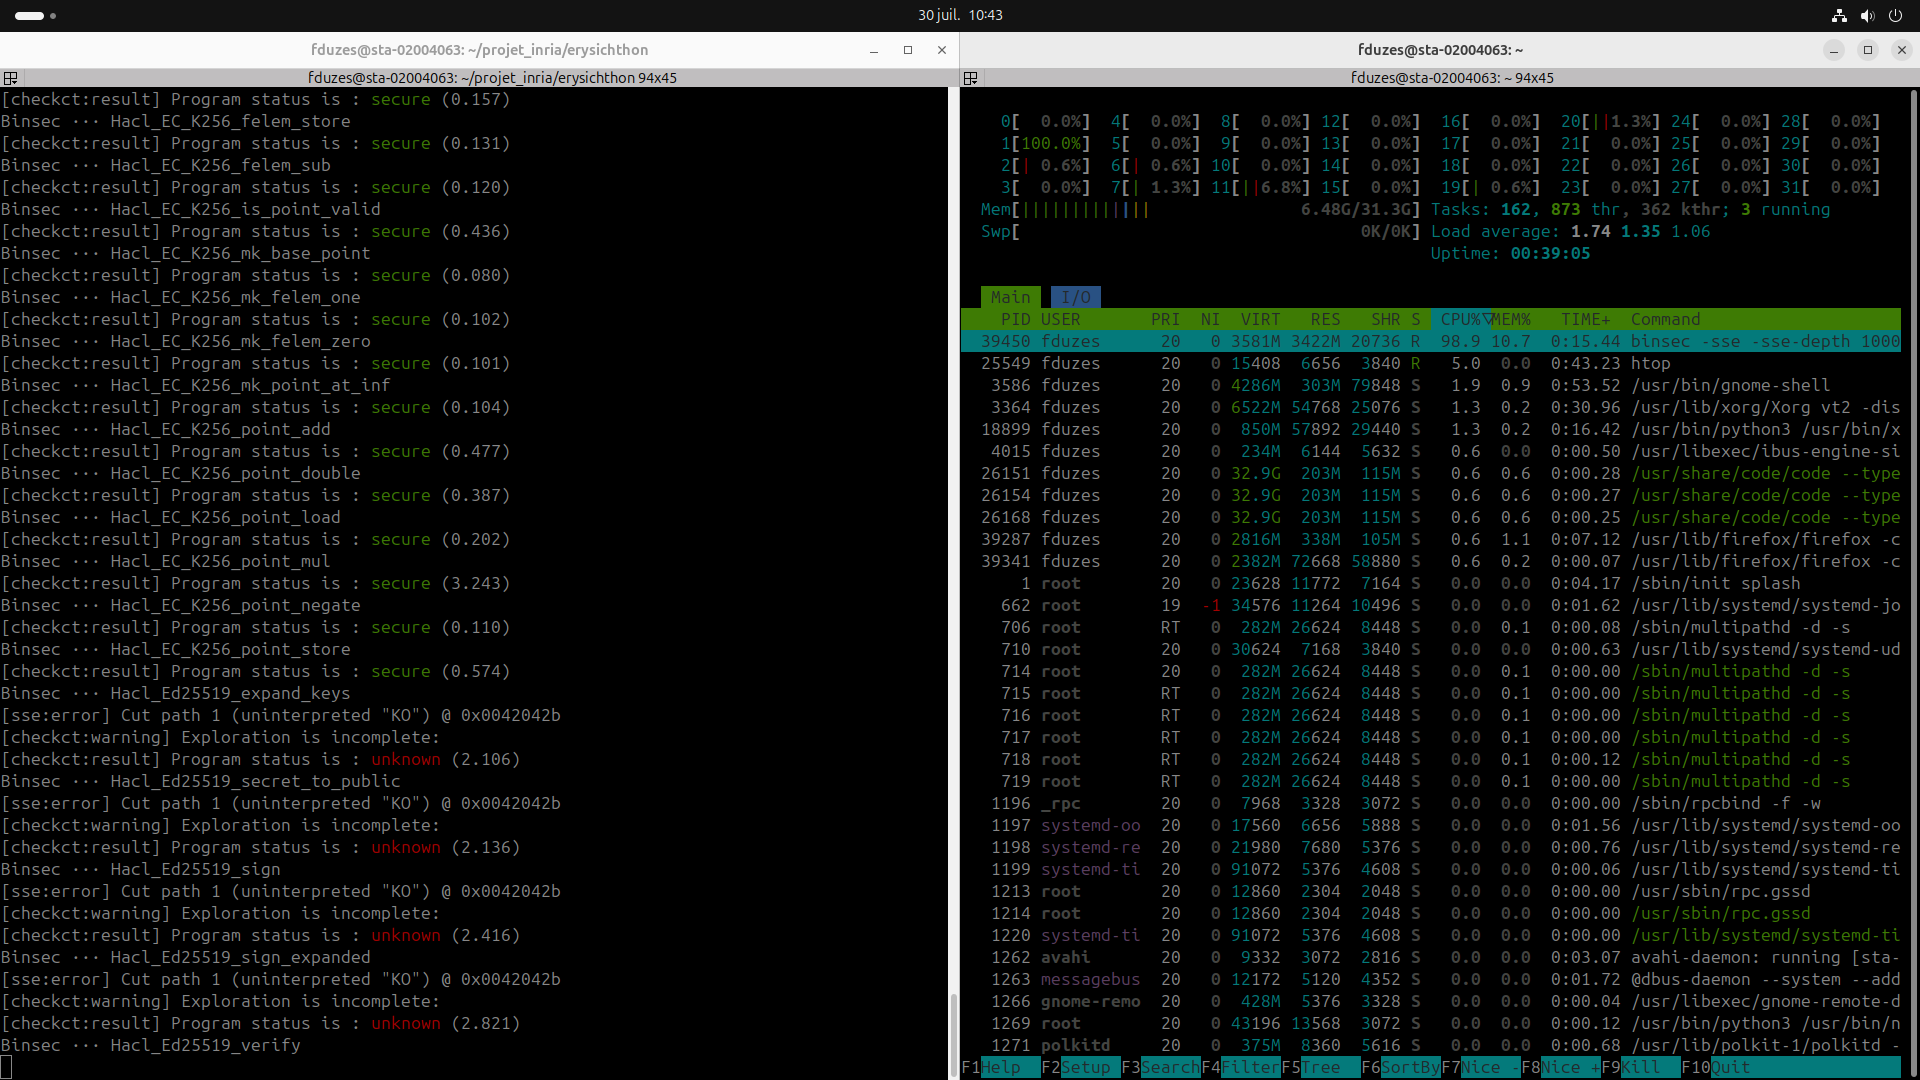
\includegraphics[scale = 0.18]{imgs/htop.png}
  \end{center}
\end{frame}

\begin{frame}[fragile]{Script Binsec}

  \begin{lstlisting}[style=INIStyle, caption={\textbf{*}.ini}, gobble=4]
    starting from core
    halt at @[rsp, 8]
    explore all
  \end{lstlisting}

\end{frame}

%%%%%%%%%%%%%%%%%%%%%%%%%%%%%%%%%%%%%%%%%%%%%%%%%%%%%%%

\section{Conclusion}
\frame{\sectionpage}

\begin{frame}{Conclusion}

  \begin{columns}
    \begin{column}{0.5\textwidth}
      \begin{block}{Erreurs binsec}
        \begin{itemize}
          \item Instructions non reconnu
          \item Syscall
        \end{itemize}
      \end{block}
    
      \begin{block}{Étendre vers les autres architectures}
        \begin{itemize}
          \item Inclure ARM et RiscV
          \item Tester sur Hacl* public
        \end{itemize}
      \end{block}
      
    \end{column}
    \pause
    \begin{column}{0.5\textwidth}
      \begin{block}{Modification de l'organisation du travail}
        \begin{itemize}
          \item Objectif \textbf{Mémoire}
          \item 5 pages par jour
          \item \textit{Continuité du projet au troisième plan}
        \end{itemize}
      \end{block}
    \end{column}
  \end{columns}
\end{frame}

%%%%%%%%%%%%%%%%%%%%%%%%%%%%%%%%%%%%%%%%%%%%%%%%%%%%%%%

%% Le texte est modifiable en changeant \thankyou
%% \renewcommand{\thankyou}{Thank You.}
\frame{\merci}


\end{document}

